

Benutzer mit Administratorrechten haben Zugriff auf den Menüpunkt \glqq Administration\grqq{}, über den sie die Benutzerverwaltung der Anwendung steuern können. 

In der Übersicht werden alle registrierten Benutzer angezeigt, inklusive:

\begin{itemize}
    \item \textbf{Benutzername}
    \item \textbf{Erstellt am (Zeitstempel)}
    \item \textbf{Rolle} (z.\,B. \texttt{Admin} oder \texttt{User})
\end{itemize}

\vspace{0.5em}
Folgende Funktionen stehen zur Verfügung:

\begin{itemize}
    \item \textbf{Benutzer löschen:} Entfernt den ausgewählten Benutzer dauerhaft aus dem System.
    \item \textbf{Passwort zurücksetzen:} Setzt das Passwort des ausgewählten Benutzers auf \glqq defaultPassword\grqq{} zurück. Nach dem Login kann der Benutzer das Passwort über die Einstellungen ändern.
    \item \textbf{Rolle zuweisen:} Ermöglicht die Zuweisung einer neuen Rolle (z.\,B. \texttt{Admin} oder \texttt{User}) an den ausgewählten Benutzer.
\end{itemize}

Diese Funktionen sind ausschließlich für Administratoren verfügbar und ermöglichen eine zentrale und sichere Verwaltung der Benutzerkonten.

Besondere Regeln gelten für zwei spezielle Fälle:

\begin{itemize}
    \item Der \textbf{erste registrierte Benutzer} erhält automatisch die Rolle \texttt{Admin}.
    \item Der Benutzer mit dem festen Benutzernamen \texttt{admin} ist dauerhaft Administrator und kann aus Sicherheitsgründen weder bearbeitet noch gelöscht werden.
\end{itemize}

Diese Schutzmechanismen stellen sicher, dass stets mindestens ein voll berechtigter Administrator vorhanden ist, der die vollständige Kontrolle über das System behält.

\begin{figure}[H]
    \centering
    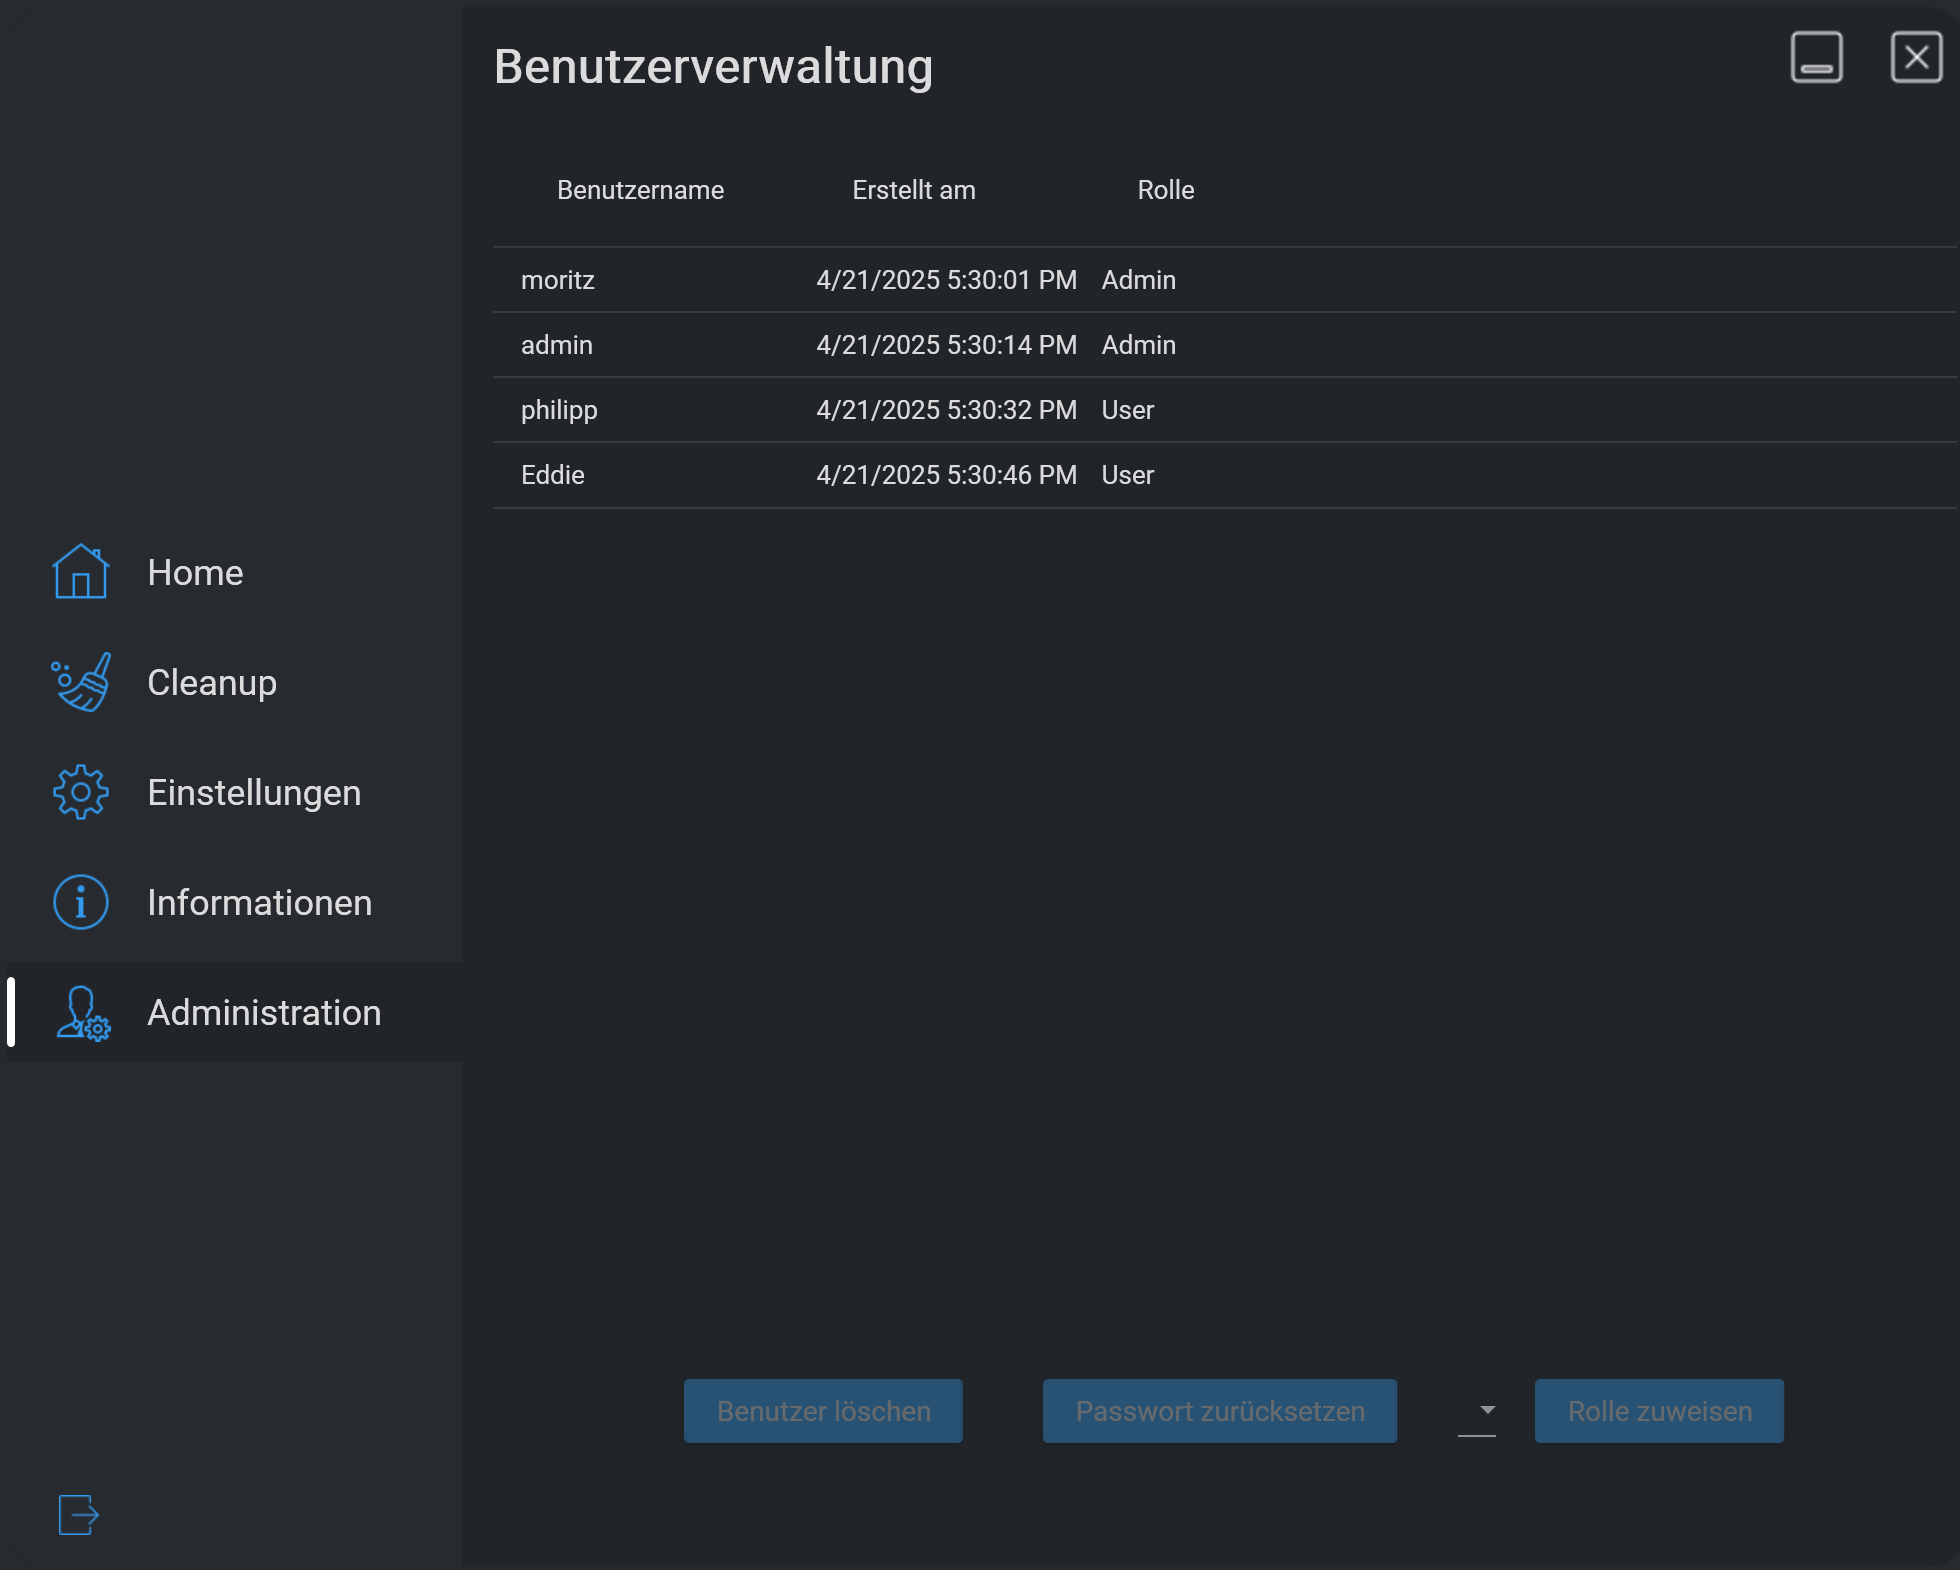
\includegraphics[width=0.9\textwidth]{src/screenshot_admin.png}
    \caption{Administrationsbereich zur Benutzerverwaltung mit Rollenzuweisung}
\end{figure}
